\chapter{P\'olya Kernels, Generalized Gamma Convolutions and Thorin Measures}\label{ch:10}

In 1926 P\'olya studied Riemann's $\Xi$ function as the Fourier transform of an explicit positive even kernel and asked which properties of a kernel force its transform to have only real zeros. For Riemann's kernel the question is the Riemann hypothesis, still open; it led to de Bruijn's heat flow and the de Bruijn Newman constant. Two later strands from probability, Thorin's generalized gamma convolutions and the Brownian identities surveyed by Biane, Pitman and Yor, supply the language of this chapter. We transport P\'olya's framework from $\zeta$ to an automorphic $L$ function of $\GL_2$. For the discriminant form $\Delta$ the kernel is $\Delta$ itself on the imaginary axis, read in logarithmic coordinates; the corresponding random variable has a characteristic function that vanishes at $t$ exactly when $L(6+it,\Delta)=0$; and the Riemann hypothesis for $\Delta$ becomes the statement that a certain reciprocal is the Laplace transform of a generalized gamma convolution with an explicit Thorin measure. We prove these equivalences in full. They reformulate the Riemann hypothesis for $\Delta$ without proving it, and we say exactly what is missing.

\section{The P\'olya kernel of the Riemann zeta function}

Let $\xi(s) = \frac12 s(s-1)\pi^{-s/2}\Gamma(s/2)\zeta(s)$ and $\Xi(t) = \xi(\frac12+it)$. Riemann \cite{riemann1859} observed that $\Xi$ is entire, even and real on $\R$, and the Riemann hypothesis\index{Riemann hypothesis} is the statement that all zeros of $\Xi$ are real. From the theta transformation formula one obtains
\begin{gather}
\Xi(t) = \int_{-\infty}^\infty \Phi(u)\,e^{itu}\,du,\label{eq:ch10polya}\\
\Phi(u) = 2\sum_{n\ge1}\bigl(2\pi^2n^4e^{9u/2} - 3\pi n^2e^{5u/2}\bigr)\exp\bigl(-\pi n^2e^{2u}\bigr).\notag
\end{gather}
The kernel $\Phi$ is even, strictly positive, and decays like $\exp(-\pi e^{2|u|}+\frac92|u|)$. After normalisation by $\Xi(0)$ it is the density of a symmetric random variable whose characteristic function is $\Xi(t)/\Xi(0)$.\index{P\'olya kernel}

P\'olya \cite{polya1926} proved that an explicit approximation of $\Phi$ built from its leading term has a transform with only real zeros, and in a sequel \cite{polya1927} he identified multipliers of a kernel, among them $e^{\lambda u^2}$ with $\lambda>0$, that preserve the reality of the zeros of its transform. De Bruijn \cite{debruijn1950} made the second idea quantitative. Put
\[
H_\lambda(z) = \int_{-\infty}^\infty e^{\lambda u^2}\Phi(u)\,e^{izu}\,du ,
\]
so that $H_0=\Xi$. If all zeros of $H_0$ lie in the strip $|\operatorname{Im}z|\le b_0$, then for $\lambda>0$ all zeros of $H_\lambda$ lie in $|\operatorname{Im}z|\le\sqrt{\max(b_0^2-2\lambda,0)}$. For $\Xi$ one may take $b_0=\frac12$, so $H_\lambda$ has only real zeros for $\lambda\ge\frac18$.\index{heat flow} Newman \cite{newman1976} showed that there is a real constant $\lambda_0$ such that $H_\lambda$ has only real zeros exactly when $\lambda\ge\lambda_0$, and conjectured $\lambda_0\ge0$; the Riemann hypothesis is the statement $\lambda_0\le0$. The literature normalises the heat flow by $H_0(z)=\frac18\Xi(z/2)$, in which the threshold is the de Bruijn Newman constant\index{de Bruijn Newman constant} $\Lambda=4\lambda_0$ and de Bruijn's bound reads $\Lambda\le\frac12$. Rodgers and Tao \cite{rodgerstao2020} proved Newman's conjecture $\Lambda\ge0$, and the Polymath project \cite{polymath2019} proved $\Lambda\le0.22$.

\subsection{The Laguerre P\'olya class and P\'olya frequency functions}

An entire function belongs to the \emph{Laguerre P\'olya class}\index{Laguerre P\'olya class} if it is a locally uniform limit of real polynomials with only real zeros; by the theorem of Laguerre and P\'olya these are the real entire functions of genus at most one with only real zeros, times a factor $e^{-\gamma z^2}$ with $\gamma\ge0$ \cite{levin1964}. The Riemann hypothesis is the statement that $\Xi$ is in the Laguerre P\'olya class. A function $f$ on $\R$ is a \emph{P\'olya frequency function}\index{P\'olya frequency function} of infinite order if every determinant $\det[f(x_i-y_j)]$ with $x_1<\dots<x_n$ and $y_1<\dots<y_n$ is nonnegative.

\begin{theorem}[Schoenberg]\label{thm:ch10schoenberg}
An integrable function $f$ on $\R$, not almost everywhere zero, is a P\'olya frequency function of infinite order if and only if its bilateral Laplace transform is $\int e^{-sx}f(x)\,dx = 1/\Psi(s)$ in a vertical strip containing the imaginary axis, with
\[
\Psi(s) = Ce^{-\gamma s^2+\delta s}\prod_k(1+\delta_ks)e^{-\delta_ks},
\]
where $C>0$, $\gamma\ge0$, $\delta,\delta_k\in\R$ and $0<\gamma+\sum_k\delta_k^2<\infty$.
\end{theorem}

The functions $\Psi$ in Schoenberg's theorem \cite{schoenberg1951,karlin1968} are exactly the members of the Laguerre P\'olya class that are positive at the origin and not of the form $Ce^{\delta s}$. Thus a real entire function $\Psi$ with $\Psi(0)>0$, equal to $e^{-\gamma s^2}$ with $\gamma\ge0$ times a function of genus at most one and not of the form $Ce^{\delta s}$, has only real zeros exactly when $1/\Psi$ is, near the imaginary axis, the bilateral Laplace transform of a P\'olya frequency function.

\section{Gamma convolutions and Thorin measures}

\begin{definition}\label{def:ch10ggc}
A probability law on $[0,\infty)$ is a \emph{generalized gamma convolution}\index{generalized gamma convolution} (GGC) if it is a weak limit of finite convolutions of gamma laws. Equivalently \cite{thorin1977,bondesson1992}, its Laplace transform is
\[
\varphi(s) = \exp\Bigl(-as - \int_{(0,\infty)}\log\Bigl(1+\frac{s}{t}\Bigr)\,\tau(dt)\Bigr),\qquad s\ge0,
\]
with $a\ge0$ and a positive measure $\tau$ on $(0,\infty)$, finite on compact sets, the \emph{Thorin measure}\index{Thorin measure}, satisfying $\int_{(0,1]}|\log t|\,\tau(dt)<\infty$ and $\int_{(1,\infty)}t^{-1}\,\tau(dt)<\infty$. These conditions say exactly that the integral in the exponent is finite for $s>0$.
\end{definition}

By Frullani's integral $\log(1+s/t) = \int_0^\infty(1-e^{-sx})e^{-tx}x^{-1}\,dx$, so a GGC is infinitely divisible with drift $a$ and L\'evy measure $k(x)x^{-1}dx$, where
\[
k(x) = \int e^{-tx}\,\tau(dt)
\]
is completely monotone. Conversely an infinitely divisible law on $[0,\infty)$ whose L\'evy measure has density $k(x)/x$ with $k$ completely monotone is a GGC, and $\tau$ is the Bernstein measure of $k$. A gamma law with shape $\alpha$ and rate $t$ has Thorin measure $\alpha\delta_t$. GGCs are self decomposable, hence unimodal, and the class is closed under convolution and weak limits \cite{bondesson1992}.

\begin{lemma}\label{lem:ch10nonvanish}
The Laplace transform of a GGC extends to a holomorphic function on $\C\setminus(-\infty,0]$ with no zeros there.
\end{lemma}

\begin{proof}
For $s$ in a compact $K\subset\C\setminus(-\infty,0]$ and $t>0$, the number $1+s/t$ avoids $(-\infty,0]$, so the principal logarithm $\log(1+s/t) = \log(t+s)-\log t$ is holomorphic in $s$. It is bounded by $2|s|/t$ for $t\ge2\max_K|s|$, by $|\log t|+C_K$ for $t\le1$, and by a constant on the compact range between. By the conditions on $\tau$ the integral converges absolutely and uniformly on $K$, so the exponent is holomorphic on $\C\setminus(-\infty,0]$, it agrees with $\log\varphi$ for $s>0$, and its exponential has no zeros.
\end{proof}

\subsection{Brownian motion and the Riemann $\xi$ function}\label{sec:ch10bpy}

Biane, Pitman and Yor \cite{bpy2001} survey a probabilistic reading of $\xi$ through Brownian motion. Let $T$ be the first hitting time of $1$ by a three dimensional Bessel process started at $0$. Then $\E e^{-\lambda T} = \sqrt{2\lambda}/\sinh\sqrt{2\lambda}$, and the product formula for $\sinh$ gives
\[
\E e^{-\lambda(T+\hat T)} = \Bigl(\frac{\sqrt{2\lambda}}{\sinh\sqrt{2\lambda}}\Bigr)^2 = \prod_{n\ge1}\Bigl(1+\frac{2\lambda}{\pi^2n^2}\Bigr)^{-2}
\]
for an independent copy $\hat T$. Hence $T+\hat T$ is a GGC with Thorin measure $2\sum_n\delta_{\pi^2n^2/2}$: it has the law of $\sum_n 2G_n/(\pi^2n^2)$ with $G_n$ independent gamma variables of shape $2$. The variable $Y = \sqrt{\pi(T+\hat T)/2}$, which has the law of $\sqrt{2/\pi}$ times the maximum of a standard Brownian excursion, satisfies
\[
\E[Y^s] = 2\xi(s)\qquad\text{for all } s\in\C .
\]
The functional equation $\xi(s)=\xi(1-s)$ becomes a distributional identity for $Y$, and the Euler product plays no role. The identity $\xi(\frac12+z)/\xi(\frac12) = \E[Y^{1/2+z}]/\E[Y^{1/2}]$ shows that P\'olya's density $\Phi/\Xi(0)$ is the density of $\log Y$ when the law of $Y$ is size biased by $Y^{1/2}$. Theorem~\ref{thm:ch10kernel} below gives the analogue for $\Delta$: $\E[(e^W)^{s-6}] = \Lambda(s,\Delta)/\Lambda(6,\Delta)$, and the functional equation is the symmetry of $W$.

\subsection{The reciprocal Xi function}

The first author \cite{polson2017} studied the reciprocal of $\Xi$ in the variable $\sqrt s$. Since $\Xi$ is even and of order one, $t\mapsto\Xi(\sqrt t)$ is entire of order one half, and if all zeros of $\Xi$ are real, say $\pm\gamma_k$ with $\gamma_k>0$, Hadamard's theorem gives
\[
\frac{\xi(\frac12)}{\xi(\frac12+\sqrt s)} = \prod_k\Bigl(1+\frac{s}{\gamma_k^2}\Bigr)^{-1},
\]
which is the Laplace transform of the GGC $\sum_kE_k/\gamma_k^2$, with $E_k$ independent standard exponential variables and Thorin measure $\sum_k\delta_{\gamma_k^2}$; conversely the GGC property forces the zeros onto the line, by the argument of Theorem~\ref{thm:ch10ggc} below. That paper develops this Thorin representation, its L\'evy measure and a transform taking the L\'evy measure of the primal function to the Thorin measure of its reciprocal, as a route to Hilbert's eighth problem. It does not prove the Riemann hypothesis, and neither does this book; what it supplies is a dictionary in which the Riemann hypothesis is a positivity statement. We now build the same dictionary for the discriminant form, where each identity can be checked numerically.

\section{The P\'olya kernel of the discriminant form}

Let $\Delta(\tau) = q\prod_{n\ge1}(1-q^n)^{24} = \sum_n\tau(n)q^n$ with $q = e^{2\pi i\tau}$, the cusp form of weight $12$ for $\SL_2(\Z)$. We use the classical normalisation of Chapter~\ref{ch:02}: $L(s,\Delta) = \sum_n\tau(n)n^{-s}$ and $\Lambda(s,\Delta) = (2\pi)^{-s}\Gamma(s)L(s,\Delta)$, which is entire with $\Lambda(s,\Delta) = \Lambda(12-s,\Delta)$ by Hecke's Theorem~\ref{thm:02fe}, so the centre is $s=6$. All zeros of $\Lambda(s,\Delta)$ lie in $\frac{11}{2}<\operatorname{Re}s<\frac{13}{2}$ (Section~\ref{sec:02mellin}; on the line $\operatorname{Re}s=\frac{13}{2}$ this is Proposition~\ref{prop:ch09nonvanish} away from $s=\frac{13}{2}$ and Proposition~\ref{prop:ch10mellin} below at $s=\frac{13}{2}$), and the Riemann hypothesis for $\Delta$ is the conjecture that they all lie on $\operatorname{Re}s=6$.

\begin{proposition}\label{prop:ch10mellin}
For all $s\in\C$,
\[
\Lambda(s,\Delta) = \int_0^\infty\Delta(iy)\,y^{s-1}\,dy,
\]
with $\Delta(iy) = e^{-2\pi y}\prod_n(1-e^{-2\pi ny})^{24}>0$ for $y>0$ and $\Delta(i/y) = y^{12}\Delta(iy)$. In particular $\Lambda(\sigma,\Delta)>0$ for real $\sigma$.
\end{proposition}

\begin{proof}
Section~\ref{sec:02mellin} gives the identity for $\operatorname{Re}s>7$. The proof of Theorem~\ref{thm:02fe} gives $\Delta(i/y) = y^{12}\Delta(iy)$ and shows that $\Delta(iy)$ decays faster than any power of $y$ at both ends, so the integral converges absolutely for every $s$ and defines an entire function, which equals $\Lambda$ by analytic continuation. Positivity of $\Delta(iy)$ is clear from the product, and for real $\sigma$ the integrand is positive.
\end{proof}

Substitute $y = e^u$. The function $g(u) = \Delta(ie^u)e^{6u}$ satisfies $g(-u) = \Delta(ie^{-u})e^{-6u} = e^{12u}\Delta(ie^u)e^{-6u} = g(u)$, and $\int g = \Lambda(6,\Delta)$.

\begin{definition}
The \emph{P\'olya kernel of $\Delta$} is the probability density
\[
\Phi_\Delta(u) = \frac{\Delta(ie^u)\,e^{6u}}{\Lambda(6,\Delta)},\qquad u\in\R,
\]
and $W$, the \emph{P\'olya variable} of $\Delta$, is a random variable with density $\Phi_\Delta$.
\end{definition}

The numbers are $L(6,\Delta) = 0.792123$ and
\[
\Lambda(6,\Delta) = 120\,L(6,\Delta)/(2\pi)^6 = 0.0015449.
\] The kernel is even, strictly positive, and decays doubly exponentially, $\Phi_\Delta(u)\asymp\exp(-2\pi e^{|u|}+6|u|)$. Figure~\ref{fig:deltakernel} compares it with the normal density of the same variance. The two are close: the peak $\Phi_\Delta(0)=1.1557$ lies below the normal peak $1.1902$, and under the Riemann hypothesis for $\Delta$ the kernel is platykurtic (Exercise~\ref{ex:ch10kurtosis}). Its tails, too small to see at this scale, are far lighter than Gaussian ones.


\begin{figure}[t]
\centering
\begin{minipage}[t]{0.48\textwidth}\centering
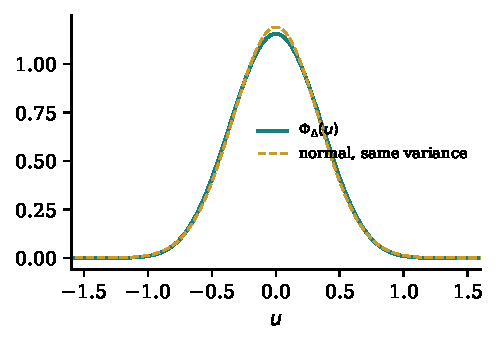
\includegraphics[width=\textwidth]{figs/deltakernel.pdf}
\caption{The kernel $\Phi_\Delta$ against the normal density with the same variance $0.112352$.}\label{fig:deltakernel}
\end{minipage}\hfill
\begin{minipage}[t]{0.48\textwidth}\centering
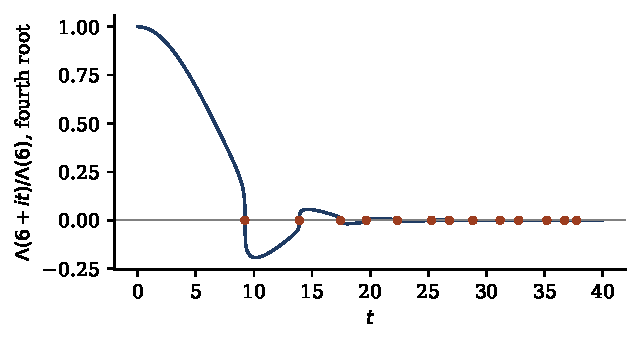
\includegraphics[width=\textwidth]{figs/deltazeros.pdf}
\caption{The characteristic function $\E e^{itW} = \Lambda(6+it,\Delta)/\Lambda(6,\Delta)$ for $0\le t\le40$, plotted as a signed fourth root to make the decaying oscillations visible, with its zeros $\gamma_k$ marked.}\label{fig:deltazeros}
\end{minipage}
\end{figure}

\begin{theorem}[this book]\label{thm:ch10kernel}
The random variable $W$ is symmetric, has moments of all orders and an entire moment generating function, and for all $z\in\C$
\[
\E\bigl[e^{zW}\bigr] = \frac{\Lambda(6+z,\Delta)}{\Lambda(6,\Delta)} .
\]
In particular $\E[e^{itW}] = \Lambda(6+it,\Delta)/\Lambda(6,\Delta)$ is real and even, and the Riemann hypothesis for $\Delta$ is equivalent to the statement that the characteristic function of $W$ has only real zeros.
\end{theorem}

\begin{proof}
By Proposition~\ref{prop:ch10mellin} for $s = 6+z$ and $y = e^u$, $\Lambda(6+z) = \int g(u)e^{zu}\,du$, which converges absolutely for all $z$ by the doubly exponential decay of $g$; dividing by $\Lambda(6)$ gives the identity. Symmetry of $\Phi_\Delta$ makes the characteristic function real and even. Zeros of $\Lambda(s,\Delta)$ are the points $6+it$ with $\E e^{itW}=0$, and they lie on $\operatorname{Re}s=6$ exactly when the corresponding $t$ is real.
\end{proof}

Our computations for this book located $404$ zeros of $\Lambda(6+it,\Delta)$ on the critical line with $0<t\le400$, the first six being
\[
9.22238,\quad 13.90755,\quad 17.44278,\quad 19.65651,\quad 22.33610,\quad 25.27464 .
\]
For the number $N(T)$ of zeros $6+i\gamma$ with $0<\gamma\le T$, the Riemann von Mangoldt formula for $\Delta$ reads $N(T) = \frac{T}{\pi}\log\frac{T}{2\pi e}+\frac{11}{4}+O(\log T)$, where the error term is $\frac1\pi\arg L(6+iT,\Delta)$ up to $O(1/T)$; the main terms give $404.3$ at $T=400$. The characteristic function computed by quadrature against $\Phi_\Delta$ agrees with $\Lambda(6+it)/\Lambda(6)$ to at least twelve significant digits at $t = 2,5,12$, and at $t=\gamma_1$ its computed value is $1.2\times10^{-17}$. Figure~\ref{fig:deltazeros} shows it.


\subsection{The Hadamard product and the variance identity}

The zeros of $\Lambda(6+z,\Delta)$ are symmetric under $z\mapsto-z$ and $z\mapsto\bar z$, since $\Lambda(6+z)$ is even and real for real $z$, and none is real, since $\Lambda(6+x)>0$. Writing a zero as $z = i\gamma$, we list one representative of each pair $\{\gamma,-\gamma\}$ with $\operatorname{Re}\gamma>0$ as $\gamma_1,\gamma_2,\dots$, with multiplicity and in order of increasing real part. The Riemann hypothesis for $\Delta$ says all $\gamma_k$ are real.

\begin{theorem}[this book]\label{thm:ch10hadamard}
Unconditionally, $\sum_k|\gamma_k|^{-2}<\infty$ and for all $z\in\C$
\[
\frac{\Lambda(6+z,\Delta)}{\Lambda(6,\Delta)} = \prod_k\Bigl(1+\frac{z^2}{\gamma_k^2}\Bigr).
\]
Consequently $\E W = 0$ and
\[
\operatorname{Var}W = 2\sum_k\frac{1}{\gamma_k^2},
\]
where the right side is real because nonreal $\gamma_k$ occur in conjugate pairs.
\end{theorem}

\begin{proof}
Since $\Delta(iy)>0$, Proposition~\ref{prop:ch10mellin} gives $|\Lambda(s)|\le\Lambda(\operatorname{Re}s)$ for every $s$. For real $\sigma\ge7$ we have $L(\sigma,\Delta)\le\sum_n|\tau(n)|n^{-7}<\infty$ and $\Gamma(\sigma)\le\sigma^\sigma$, and $\Lambda(\sigma) = \Lambda(12-\sigma)$; hence $|\Lambda(6+z)|\le\Lambda(6+|\operatorname{Re}z|)\le C\exp\bigl((|z|+7)\log(|z|+7)\bigr)$, and $\Lambda(6+z)$ is entire of order at most one. Define $G(w) = \Lambda(6+\sqrt w)/\Lambda(6)$. It is well defined because $\Lambda(6+z)$ is even, it is entire because an even power series in $z$ is a power series in $w = z^2$, and $|G(w)|\le C'\exp\bigl((|w|^{1/2}+7)\log(|w|^{1/2}+7)\bigr)$, so $G$ has order at most one half (exactly one half, by Stirling's formula on the real axis). Its zeros are the points $w_k = -\gamma_k^2$, with multiplicity, and $G(0) = 1$. An entire function of order less than one has genus zero, so Hadamard's theorem gives $G(w) = \prod_k(1-w/w_k)$ with $\sum_k|w_k|^{-1}<\infty$, with no exponential factor and with constant $G(0)=1$. This is the convergence statement and, with $w = z^2$, the product formula. Finally $G(w) = \E[e^{\sqrt wW}] = \sum_n\E[W^{2n}]w^n/(2n)!$ since odd moments vanish, so $G'(0) = \frac12\E W^2$, while the absolutely convergent product gives $G'(0) = \sum_k\gamma_k^{-2}$.
\end{proof}

The variance identity equates a moment of the kernel with a sum over zeros, a trace formula in miniature. Quadrature against $\Phi_\Delta$ gives $\operatorname{Var}W = 0.112352$. The $404$ computed zeros give $2\sum_{\gamma_k\le400}\gamma_k^{-2} = 0.104146$. The density of zeros at height $t$ is $\frac1\pi\log\frac{t}{2\pi}$, so the tail $\sum_{\gamma_k>T}\gamma_k^{-2}$ is approximately $\int_T^\infty\frac{\log(t/2\pi)}{\pi t^2}\,dt = \frac{\log(T/2\pi)+1}{\pi T}$, which at $T = 400$ is $0.004101$; doubling and adding gives $0.112348$, a relative difference of $3\times10^{-5}$.

\section{The Riemann hypothesis for $\Delta$ as a GGC property}

\begin{theorem}[this book]\label{thm:ch10ggc}
The following are equivalent.
\begin{enumerate}
\item[(i)] All zeros of $\Lambda(s,\Delta)$ lie on the line $\operatorname{Re}s = 6$.
\item[(ii)] The function $s\mapsto\Lambda(6,\Delta)/\Lambda(6+\sqrt s,\Delta)$, $s>0$, is the Laplace transform of a generalized gamma convolution.
\end{enumerate}
When they hold, the GGC has drift $0$ and Thorin measure $\sum_k\delta_{\gamma_k^2}$, it is the law of
\[
X = \sum_k\frac{E_k}{\gamma_k^2}
\]
with $E_k$ independent standard exponential variables, and its L\'evy measure has density
\[
\frac{k(x)}{x},\qquad k(x) = \sum_ke^{-\gamma_k^2x},
\]
which is completely monotone.
\end{theorem}

\begin{proof}
Let $G$ be as in the proof of Theorem~\ref{thm:ch10hadamard}, so the function in (ii) is $1/G(s)$ for $s>0$.

(ii) implies (i). Let $\varphi$ be the Laplace transform of the GGC. By Lemma~\ref{lem:ch10nonvanish}, $\varphi$ is holomorphic and zero free on $\C\setminus(-\infty,0]$. The function $\varphi G$ is holomorphic on this connected domain and equals $1$ on $(0,\infty)$, hence everywhere by the identity theorem, so $G$ has no zeros off $(-\infty,0]$. The zeros of $G$ are the points $-\gamma_k^2$, and $G(0) = 1$, so every $\gamma_k^2$ is a positive real number. As $\operatorname{Re}\gamma_k>0$, every $\gamma_k$ is real, and the zeros $6\pm i\gamma_k$ lie on $\operatorname{Re}s=6$.

(i) implies (ii). If all $\gamma_k$ are real, hence positive, Theorem~\ref{thm:ch10hadamard} gives $1/G(s) = \prod_k(1+s/\gamma_k^2)^{-1}$ for $s>0$. Each factor is the Laplace transform of $E_k/\gamma_k^2$. Since $\sum_k\E[E_k/\gamma_k^2] = \sum_k\gamma_k^{-2}<\infty$, the series $X$ converges almost surely and in $L^1$, and by independence and dominated convergence its Laplace transform is the infinite product. Writing the product as $\exp(-\sum_k\log(1+s/\gamma_k^2))$ exhibits it in the form of Definition~\ref{def:ch10ggc} with $a = 0$ and $\tau = \sum_k\delta_{\gamma_k^2}$. The conditions on $\tau$ hold: $\sum_k\gamma_k^{-2}<\infty$ leaves only finitely many atoms $\gamma_k^2$ below any bound, so $\tau$ is finite on compact sets and $\int_{(0,1]}|\log t|\,\tau(dt)$ is a finite sum, while $\int t^{-1}\,\tau(dt) = \sum_k\gamma_k^{-2}<\infty$. Frullani's integral gives the L\'evy density. The series $k(x)$ converges for $x>0$ because $e^{-\gamma_k^2x}\le(\gamma_k^2x)^{-1}$, and $k$ is completely monotone as the Laplace transform of the positive measure $\tau$.
\end{proof}

The first Thorin atoms are
\[
\gamma_k^2 = 85.05,\quad 193.42,\quad 304.25,\quad 386.38,\quad 498.90,\quad 638.81 .
\] Figure~\ref{fig:ggc} compares the product over the computed zeros, with the tail correction of the previous section in the exponent, to the exact value $\Lambda(6)/\Lambda(6+\sqrt s)$. The pairs (exact, corrected product over the $404$ zeros) are $(0.945467, 0.945468)$ at $s=1$, $(0.575602, 0.575612)$ at $s=10$, $(0.0069732, 0.0069741)$ at $s=100$ and $(5.6354, 5.6359)\times10^{-8}$ at $s=400$: a relative error below $2\times10^{-4}$ over more than seven orders of magnitude. Figure~\ref{fig:levydelta} shows $k$; under the Riemann hypothesis for $\Delta$, $k(x)/x$ is the L\'evy density. As $x\to0$ the zero density $\frac1\pi\log\frac{t}{2\pi}$ gives
\[
k(x) = \frac{\log(1/x)-c_0+o(1)}{4\sqrt{\pi x}},\qquad c_0 = \log(16\pi^2)+\gamma_{\mathrm E} = 5.639,
\]
with $\gamma_{\mathrm E}$ Euler's constant. The constant matters at the scale of Figure~\ref{fig:levydelta}: at $x=10^{-4}$ the numerator is about $3.57$, against $9.21$ for $\log(1/x)$ alone. The L\'evy density therefore behaves like $x^{-3/2}\log(1/x)/(4\sqrt\pi)$ at the origin: the L\'evy measure is infinite, while its first moment near the origin, $\int_0^1k(x)\,dx$, is finite, as for every subordinator.



\begin{figure}[t]
\centering
\begin{minipage}[t]{0.48\textwidth}\centering
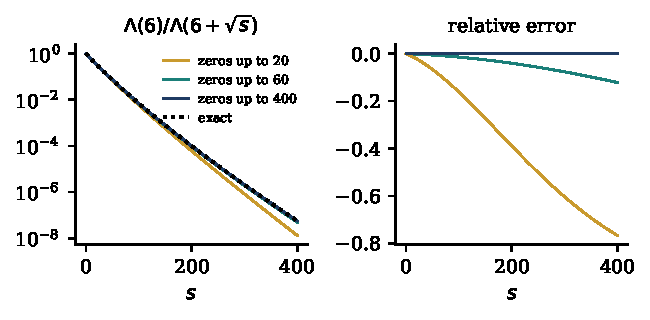
\includegraphics[width=\textwidth]{figs/ggc.pdf}
\caption{Left: the product $\prod_k(1+s/\gamma_k^2)^{-1}$ over the zeros up to height $20$, $60$ and $400$, each with its tail correction, against $\Lambda(6,\Delta)/\Lambda(6+\sqrt s,\Delta)$ (log scale). Right: the relative errors.}\label{fig:ggc}
\end{minipage}\hfill
\begin{minipage}[t]{0.48\textwidth}\centering
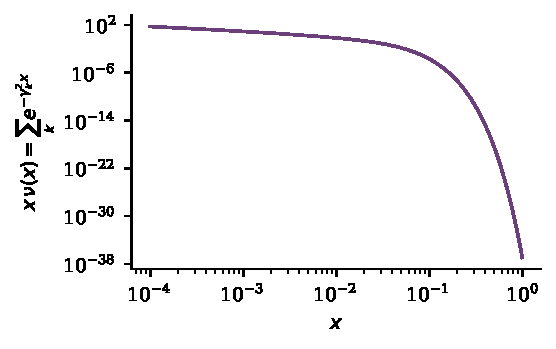
\includegraphics[width=\textwidth]{figs/levydelta.pdf}
\caption{The function $k(x) = \sum_k e^{-\gamma_k^2x}$ over the $404$ zeros up to height $400$, for $10^{-4}\le x\le1$ on log scales; under the Riemann hypothesis for $\Delta$ it is $x\nu(x)$, with $\nu$ the L\'evy density.}\label{fig:levydelta}
\end{minipage}
\end{figure}

\begin{remark}[A dual pair]\label{rem:ch10dual}
Under the Riemann hypothesis for $\Delta$ let $V = \sqrt{2X}\,N$ with $N$ standard normal independent of $X$. Then $\E e^{itV} = \E e^{-t^2X} = \Lambda(6)/\Lambda(6+t)$ for real $t$: on the real axis, the reciprocal of the moment generating function of $W$ is the characteristic function of $V$. The bilateral Laplace transform of $V$ is $1/\prod_k(1-s^2/\gamma_k^2)$ in the strip $|\operatorname{Re}s|<\gamma_1$, so by Theorem~\ref{thm:ch10schoenberg}, with $\delta_k = \pm\gamma_k^{-1}$, the density of $V$ is a P\'olya frequency function of infinite order. Conversely, if $\Lambda(6)/\Lambda(6+t)$ were the characteristic function of a P\'olya frequency density, Schoenberg's theorem would put $\prod_k(1-s^2/\gamma_k^2)$ in the Laguerre P\'olya class and all $\gamma_k$ would be real.
\end{remark}

\subsection{General self dual $L$ functions and the rank}

Apart from the variance identity, the proofs of Theorems~\ref{thm:ch10hadamard} and~\ref{thm:ch10ggc} used only that $\Lambda(6+z)$ is entire of order at most one, even, real on the real axis and nonzero at $z=0$; positivity of the kernel served only to bound the order quickly and to give the probabilistic reading of Theorem~\ref{thm:ch10kernel}. Let $\pi$ be a self dual cuspidal automorphic representation of $\GL_n(\A_\Q)$, $n\ge2$, with completed $L$ function $\Lambda(s,\pi)$ in the unitary normalisation, conductor included, so that $\Lambda(s,\pi)$ is entire of order one \cite{godementjacquet1972} and $\Lambda(s,\pi) = \varepsilon\Lambda(1-s,\pi)$ with $|\varepsilon|=1$. Self duality makes $\Lambda(s,\pi)$ real on the real axis, and then $\varepsilon=\pm1$.

\begin{theorem}[this book]\label{thm:ch10general}
Suppose $\Lambda(\frac12,\pi)\ne0$. Then the generalized Riemann hypothesis for $\pi$ holds if and only if $s\mapsto\Lambda(\frac12,\pi)/\Lambda(\frac12+\sqrt s,\pi)$ is the Laplace transform of a GGC, and then its Thorin measure is $\sum_k\delta_{\gamma_k^2}$ over the ordinates $\gamma_k>0$ of the zeros $\frac12\pm i\gamma_k$.
\end{theorem}

\begin{proof}
Since $\Lambda(\frac12)\ne0$ the functional equation at $s=\frac12$ forces $\varepsilon = 1$, so $\Lambda(\frac12+z)$ is even, and by the paragraph before the theorem the proofs of Theorems~\ref{thm:ch10hadamard} and~\ref{thm:ch10ggc} apply to $G(w) = \Lambda(\frac12+\sqrt w)/\Lambda(\frac12)$. The one new case is a real zero $\frac12+x$ of $\Lambda$, which would give a zero $x^2>0$ of $G$; the GGC property excludes it too. Theorem~\ref{thm:10babstract} gives the general argument and the other equivalent forms.
\end{proof}

When $\Lambda(\frac12+z,\pi)$ vanishes to order $r\ge1$ at $z=0$, the functional equation forces $\varepsilon=(-1)^r$, the argument applies to the even function $\Lambda(\frac12+z,\pi)/z^r$, and under the generalized Riemann hypothesis $1/\Lambda(\frac12+\sqrt s,\pi)$ is a constant times $s^{-r/2}$ times a GGC transform. The factor $s^{-r/2}$ is a degenerate Thorin atom of mass $r/2$ at the origin\index{Thorin atom at zero}, half the analytic rank for an elliptic curve; Proposition~\ref{prop:10brank} proves this, and Chapter~\ref{ch:10b} extends Theorem~\ref{thm:ch10general} to every cuspidal $\pi$, self dual or not.

\section{What is known unconditionally}

The product of Theorem~\ref{thm:ch10hadamard} splits as
\[
\frac{\Lambda(6,\Delta)}{\Lambda(6+\sqrt s,\Delta)} = \prod_{\gamma_k\in\R}\Bigl(1+\frac{s}{\gamma_k^2}\Bigr)^{-1}\times\prod_{\gamma_k\notin\R}\Bigl(1+\frac{s}{\gamma_k^2}\Bigr)^{-1}.
\]
The first factor is always a GGC transform, the law of $\sum E_k/\gamma_k^2$ over real $\gamma_k$. The second collects off line zeros in conjugate pairs. For one pair write $\gamma^2 = a+ib$ with $b\ne0$; then for $s>-a$
\begin{align*}
\Bigl(1+\frac{s}{\gamma^2}\Bigr)^{-1}\Bigl(1+\frac{s}{\bar\gamma^2}\Bigr)^{-1} &= \frac{|\gamma|^4}{(s+a)^2+b^2}\\
&= \int_0^\infty e^{-sx}\,\frac{|\gamma|^4}{b}\,e^{-ax}\sin(bx)\,dx,
\end{align*}
the Laplace transform of a function that changes sign. The Riemann hypothesis for $\Delta$ is the statement that the signed part is empty.

How much of the Thorin measure is known to be positive? Hafner \cite{hafner1983} proved, following the method of Selberg for $\zeta$ \cite{selberg1942}, that a positive proportion of the zeros of the $L$ function of a holomorphic Hecke eigenform for $\SL_2(\Z)$, counted by height, lie on the critical line. In our language, a positive proportion of the atoms $\gamma_k^2$ lie on $(0,\infty)$. But no proportion short of all of them yields the GGC property, because a single conjugate pair of nonreal $\gamma$ already destroys it, by Theorem~\ref{thm:ch10ggc}. For $\zeta$ the proportion is above two fifths \cite{conrey1989}, with the same caveat.

The heat flow transfers as well. Put $H^\Delta_\lambda(z) = \int e^{\lambda u^2}\Phi_\Delta(u)e^{izu}\,du$, so that $H^\Delta_0(z) = \Lambda(6+iz)/\Lambda(6)$. All zeros of $H^\Delta_0$ lie in $|\operatorname{Im}z|<\frac12$, so by de Bruijn's theorem $H^\Delta_\lambda$ has only real zeros for $\lambda\ge\frac18$. Dobner \cite{dobner2021}, by a method different from that of Rodgers and Tao, proved that every member of the extended Selberg class has a de Bruijn Newman constant and that it is nonnegative. The function $L(s,\Delta)$, in the unitary normalisation, belongs to that class, and Dobner's heat parameter is $4\lambda$ in our normalisation. Hence there is a constant $\lambda_\Delta$ with $0\le\lambda_\Delta\le\frac18$ such that $H^\Delta_\lambda$ has only real zeros exactly when $\lambda\ge\lambda_\Delta$, and the Riemann hypothesis for $\Delta$ is the statement $\lambda_\Delta=0$; Dobner's constant for $\Delta$ is $4\lambda_\Delta$, as $\Lambda=4\lambda_0$ for $\zeta$.\index{de Bruijn Newman constant}

\begin{remark}
Why is this a reformulation and not a proof? Every equivalence above passes through the Hadamard product, that is, through the zeros themselves. A proof of the Riemann hypothesis along these lines would need an independent construction of a GGC with Laplace transform $\Lambda(6)/\Lambda(6+\sqrt s)$, for example a stochastic process whose hitting times or occupation laws have that transform, as the Bessel hitting time $T$ of Section~\ref{sec:ch10bpy} has the transform $\sqrt{2\lambda}/\sinh\sqrt{2\lambda}$, a GGC whose Thorin atoms $\pi^2n^2/2$ come from the zeros $\pm i\pi n$ of $\sinh z/z$ (Exercise~\ref{ex:ch10bessel}). The Euler product gives positivity of a different kind, the infinite divisibility of Chapter~\ref{ch:09}, which holds only to the right of the critical strip and, for $\Delta$, holds for the Rankin Selberg function $L(s,\Delta\times\Delta)$ but not for $L(s,\Delta)$ itself: the logarithmic coefficients of $L(s,\Delta)$ change sign, and for $\sigma>\frac{13}{2}$ the function $t\mapsto L(\sigma+it,\Delta)/L(\sigma,\Delta)$ is not even a characteristic function (Proposition~\ref{prop:ch09notcf}). The GGC property is a positivity statement about the reciprocal inside the strip, and no bridge between the two is known.
\end{remark}

\begin{problem}[Hilbert's eighth problem for $\GL_2$]
Construct, without reference to the zeros, a random variable whose Laplace transform is $\Lambda(6,\Delta)/\Lambda(6+\sqrt s,\Delta)$ and prove that it is a GGC; more generally do this for every self dual cuspidal $\pi$ with $\Lambda(\frac12,\pi)\ne0$. A positive solution for one $\pi$ would prove the generalized Riemann hypothesis for that $\pi$.
\end{problem}

\section{Notes}

P\'olya's kernel and real zero theorems are in \cite{polya1926,polya1927}, the heat flow in \cite{debruijn1950,newman1976,rodgerstao2020,polymath2019}, its extension to the extended Selberg class in \cite{dobner2021}, and total positivity in \cite{schoenberg1951,karlin1968}. Thorin \cite{thorin1977,thorin1977b} introduced generalized gamma convolutions to prove that the Pareto and lognormal laws are infinitely divisible, and Bondesson's monograph \cite{bondesson1992} is the standard reference. The Brownian interpretation of $\xi$ and its relatives is the subject of the survey of Biane, Pitman and Yor \cite{bpy2001}. The Thorin representation of the reciprocal $\Xi$ function is from the first author \cite{polson2017}, and his later paper \cite{polson2018vdp} proves the equivalence of real zeros and the Thorin property for real entire functions of order at most one, with applications to Dirichlet and modular $L$ functions. Theorems~\ref{thm:ch10kernel}, \ref{thm:ch10hadamard}, \ref{thm:ch10ggc} and \ref{thm:ch10general} are elementary consequences of Hecke's theory and Hadamard's factorisation, and we present them as the book's formulation of P\'olya's programme for $\GL_2$. The numerical values were computed for this book with PARI/GP; the first zeros and $L(6,\Delta)$ agree with those listed in the LMFDB \cite{lmfdb}.

\section{Exercises}

\begin{enumerate}
\item\label{ex:ch10kurtosis} Show that $\E W^4 - 3(\E W^2)^2 = -12\sum_k\gamma_k^{-4}$, so that under the Riemann hypothesis for $\Delta$ the kernel $\Phi_\Delta$ is platykurtic. Compare with Figure~\ref{fig:deltakernel}.
\item\label{ex:ch10bessel} Let $T$ be the hitting time of $1$ by a three dimensional Bessel process from $0$. Show that $T$ is a GGC with Thorin measure $\sum_n\delta_{\pi^2n^2/2}$. Writing $\E e^{-\lambda T} = 1/F(\sqrt{2\lambda})$ with $F(z) = \sinh z/z$, explain why this is the exact analogue of Theorem~\ref{thm:ch10ggc} for an entire function whose zeros $\pm i\pi n$ are known to lie on a line.
\item\label{ex:ch10stieltjes} Show that if $\varphi$ is the Laplace transform of a GGC with drift $a$ and Thorin measure $\tau$ then $-\varphi'/\varphi = a+\int(t+s)^{-1}\tau(dt)$ is a Stieltjes function, that is, a function of the form $c/s+b+\int_{(0,\infty)}(s+t)^{-1}\sigma(dt)$ with $b,c\ge0$ and $\sigma$ a positive measure satisfying $\int(1+t)^{-1}\sigma(dt)<\infty$, hence completely monotone. Deduce that under the Riemann hypothesis for $\Delta$ the function $\frac{d}{ds}\log G(s) = \sum_k(s+\gamma_k^2)^{-1}$ is a Stieltjes function.
\item\label{ex:ch10cm} Show conversely that if $\frac{d}{ds}\log G$ agrees on a half line $(s_0,\infty)$ with a Stieltjes function then the Riemann hypothesis for $\Delta$ holds. (A Stieltjes function extends holomorphically to $\C\setminus(-\infty,0]$.) Show also that $\frac{d}{ds}\log G(s)$ is the Laplace transform of $k$ for $s>\frac14$, where $k(x) = \sum_ke^{-\gamma_k^2x}$ is defined unconditionally with complex $\gamma_k$ taken in conjugate pairs (note $|\operatorname{Im}\gamma_k|<\frac12$, so $\operatorname{Re}\gamma_k^2>-\frac14$), and conclude by Bernstein's theorem that the Riemann hypothesis for $\Delta$ is equivalent to complete monotonicity of $k$ on $(0,\infty)$.
\item Verify Remark~\ref{rem:ch10dual}: if $X$ is a GGC with Thorin measure $\sum\delta_{\gamma_k^2}$ and $V = \sqrt{2X}N$, then $V$ has the law of $\sum_kL_k/\gamma_k$ with independent standard Laplace $L_k$.
\end{enumerate}

\section{Open computational problems}

\begin{compproblem}[The Thorin measure of $\Delta$ to height $10^5$]
Objective: compute the zeros of $\Lambda(6+it,\Delta)$ for $0<t\le10^5$ and estimate the Thorin measure and the L\'evy density of Theorem~\ref{thm:ch10ggc}. Objects and scale: about $2.8\times10^5$ zeros. Route: PARI/GP \texttt{lfunzeros} or Rubinstein's \texttt{lcalc} with $\tau(n)$ precomputed to the needed length, with Turing's method to certify the count; the Mellin integral by which Chapter~\ref{ch:scholze} evaluates $\Lambda(s,\Delta)$ needs a working precision that grows with $t$ and is no route at this height. Deliverable: the zero list, the empirical measure $\sum\delta_{\gamma_k^2}$ against its smooth prediction, $k(x)$ on a logarithmic grid with tail corrections, and the convergence of $2\sum\gamma_k^{-2}$ and $-12\sum\gamma_k^{-4}$ to the cumulants $\kappa_2$ and $\kappa_4$ of $W$ computed from the kernel. Why it matters: it verifies the Riemann hypothesis for $\Delta$ to height $10^5$ and shows, in the GGC language, how fast the truncated Thorin measures reproduce the kernel.
\end{compproblem}

\begin{compproblem}[The de Bruijn Newman constant of $\Delta$]
Objective: bound $\lambda_\Delta$ from above by running the heat flow $H^\Delta_\lambda$ numerically. Objects and scale: $\lambda\in[0,\frac18]$, zeros of $H^\Delta_\lambda$ to height $10^4$, with a barrier argument in the style of the Polymath project for larger heights. Route: an effective approximation of $H^\Delta_\lambda$ by sums over $\tau(n)$, derived as the Polymath project did for $\zeta$ and evaluated in Arb with GPU parallelism over $z$; direct quadrature of $e^{\lambda u^2}\Phi_\Delta(u)\cos(zu)$ as a check at small $z$, where cancellation is mild. Deliverable: a certified upper bound $\lambda_\Delta\le\bar\lambda$ with $\bar\lambda$ well below $\frac18$, and plots of zero trajectories. Why it matters: since $\lambda_\Delta\ge0$ is known, the Riemann hypothesis for $\Delta$ is the statement $\lambda_\Delta=0$, and $\bar\lambda$ measures how close unconditional knowledge comes to it, as the bound $\Lambda\le0.22$, that is $\lambda_0\le0.055$ in our normalisation, does for $\zeta$.
\end{compproblem}

\begin{compproblem}[Monotonicity across weights and levels]
Objective: test, for many forms, that $k(x) = \sum_ke^{-\gamma_k^2x}$ is completely monotone and that $\frac{d}{ds}\log G(s)$ is a Stieltjes function, using data that do not presuppose the zeros: $k$ computed from the primes through the explicit formula, and $\frac{d}{ds}\log G$ from values of $\Lambda$. (A $k$ assembled from zeros located on the critical line is completely monotone by construction, so that test would be empty.) For $\Delta$, Table~\ref{tab:10dheat} and Figure~\ref{fig:10dheatfig} of Chapter~\ref{ch:10d} compute $k$, there written $\mathcal W$, and its first three derivatives from the primes; the problem concerns the other forms. Objects and scale: all other newforms with rational coefficients and trivial character, of weight at most $24$ and level $N\le500$, with nonzero central value, from LMFDB. Route: compute $\Lambda$ at the centre plus $\sqrt s$ with PARI/GP \texttt{lfun} on a grid $s\in[0,10^4]$, and $k$ and its derivatives from the explicit formula with Gaussian test functions; test the first twenty sign conditions $(-1)^nk^{(n)}\ge0$ in multiprecision, and fit a positive measure $\sigma$ in $\frac{d}{ds}\log G(s) = \int(s+t)^{-1}\sigma(dt)$ by nonnegative least squares. Deliverable: a table of forms with the smallest margin found in each inequality and the fitted Thorin measures compared with the squared zero ordinates. Why it matters: complete monotonicity of $k$ and the Stieltjes property are each equivalent to the generalized Riemann hypothesis for the form (Exercises~\ref{ex:ch10stieltjes} and~\ref{ex:ch10cm} for $\Delta$, with the same proofs in general), and the margins measure the distance to the boundary of the GGC cone.
\end{compproblem}

\begin{compproblem}[Rank two curves and the degenerate atom]
Objective: exhibit the degenerate Thorin atom of mass $r/2$ at the origin for elliptic curves of analytic rank $r=2$. Objects and scale: the first fifty curves of analytic rank two in LMFDB by conductor, starting with 389a1, with zeros to height $10^3$. Route: PARI/GP \texttt{lfun} and \texttt{lfunzeros} in the classical normalisation with centre $1$; evaluate $\frac{d}{ds}\log\Lambda(1+\sqrt s,E)$ on $s\in[10^{-4},10^3]$ and fit the representation $m/s+\int(s+t)^{-1}\tau(dt)$ with $m\ge0$ and $\tau\ge0$ by regularised nonnegative least squares. Deliverable: the fitted mass near $t=0$ against the predicted value $r/2 = 1$ (that is, the coefficient $m$ of $1/s$), and the remainder of the measure against $\sum\delta_{\gamma_k^2}$. Why it matters: it checks the dictionary between order of vanishing and Thorin mass at zero by fitting the whole measure, not only the slope near $s=0$ that Chapter~\ref{ch:10b} reports for 389a1.
\end{compproblem}
